\section{Experiments and Results}
\label{sec:Experiments}

\begin{comment}
Trying and failing is a major part of research.
However, to have a chance of success you need a plan driving the experimental research.
So first decide what experiments or series of experiments you plan --- and describe them in this section.
\end{comment}

In this section I will elaborate on my approach when training models, before presenting the most important findings from my experiments.

\subsection{Experimental Setup}
\label{sec:experimentalSetup}

% The experimental setup should include all data --- parameters, etc. --- that would allow a person to repeat your experiments.

All experiments were performed on an NVIDIA GeForce RTX 4090, having 24 GB G6X memory\footnote{\url{https://www.nvidia.com/nb-no/geforce/graphics-cards/40-series/rtx-4090/}}. Computing resources belong to the Department of Geomatics at NTNU and are shared with fellow 5th year geomatics students. PyTorch\footnote{\url{https://pytorch.org/}} was used to create a training loop, and Huggingface's \texttt{transformers} library was used to fetch pre-trained models from their hub.

The best results of \cite{scherrerHeLjuVarDial20202020} came from using a language-specific \acrshort{acr:bert}. As no pre-trained model was found in \citeyear{scherrerHeLjuVarDial20202020}, they fine-tuned the pre-trained \texttt{bert-base-german-uncased}\footnote{\url{https://huggingface.co/bert-base-german-uncased}} model on the SwissCrawl corpus \citep[3-4]{scherrerHeLjuVarDial20202020}. Since then, a pre-trained Swiss \acrshort{acr:bert} model\footnote{\url{https://huggingface.co/statworx/bert-base-german-cased-finetuned-swiss}} has been released, which I used in my experiments.

Becuase of the limited timespan and computing resources of this project, I opted to freeze certain of \citeauthor{scherrerHeLjuVarDial20202020}'s hyperparameters. This includes the maximum sequence length and the batch size, the latter of which was also limited by the GPU memory. The loss function (MAE/L1) and scaler (joint \citep[5]{scherrerHeLjuVarDial20202020}) also largely remained unchanged. The focus of my experiments was to compare performance of pre-trained model, and seeing what effect different coordinate projections and learning rates have.

\subsection{Experimental Results}
\label{sec:experimentalResults}

\begin{comment}
Results should be clearly displayed and should provide a suitable representation of your results for the points you wish to make.
Graphs should be labeled in a legible font. If more than one result is displayed in the same graph, then these should be clearly marked.
Please choose carefully rather than presenting every result.
Too much information is hard to read and often hides the key information you wish to present.
Make use of statistical methods when presenting results, where possible to strengthen the results.
Further, the format of the presentation of results should be chosen based on what issues in the results you wish to highlight.
You may wish to present a subset in the experimental section and provide additional results in an appendix.
If there are specific points related to one experiment that you want to discuss in more detail, it could be reasonable to do
that already in this section; however, save the main overall discussion for Section~\ref{sec:Discussion}.
\end{comment}

A total of 15 models were trained. \autoref{tbl:highlighted-results} shows a selection of the most interresting results along with to coordinate projection and learning rate/learning rate scheduler used. A full overview of configurations and their corresponding results can be found on the project's \href{https://github.com/oskarhlm/TDT13}{GitHub page}. Fine-tuned models and training logs can be found in this \href{https://drive.google.com/drive/folders/1-6nAdhvf5DBHtWzpZa6iH7z0dFETi80h?usp=sharing}{Google Drive folder}.

The best results were achieved when using the \texttt{statworx/bert-base-german-cased-finetuned-swiss} pre-trained model with a reduced development/validation dataset. Learning rate schedulers did not prove very efficient for this task and a low learning rate of 2e-5 yielded the best results instead. No real differnece in performance was observed when using the UTM projection over raw latitude/longitude values, but the Swiss-native LV95 projection gave the model a performance boost into the 15-kilometer range. The X-Mod based \texttt{swissbert} model did not prove efficient for the task at hand.

\autoref{fig:pointwise-distance} show the pointwise distance from the ground truth when using the best-performing model to make predictions on the test gold dataset.

\begin{table}
    \centering
    \begin{tabular}{p{0.3\textwidth}|p{0.12\textwidth}|p{0.22\textwidth}|p{0.22\textwidth}}
        \toprule
        Pre-trained model                                        & Coordinate Projection & LR/Scheduler      & Median Distance [km] \\
        \midrule
        dbmdz/\textbf{bert-base-german-uncased}                  & lat/lon               & 4e-5              & 17.81                \\
        statworx/\textbf{bert-base-german-cased-finetuned-swiss} & lat/lon               & 4e-5              & 17.08                \\
        statworx/\textbf{bert-base-german-cased-finetuned-swiss} & UTM                   & ReduceLROnPlateau & 16.52*               \\
        statworx/\textbf{bert-base-german-cased-finetuned-swiss} & UTM                   & 2e-5              & 16.05*               \\
        statworx/\textbf{bert-base-german-cased-finetuned-swiss} & lat/lon               & 2e-5              & 16.19*               \\
        statworx/\textbf{bert-base-german-cased-finetuned-swiss} & LV95                  & 2e-5              & \textbf{15.76}*      \\
        ZurichNLP/\textbf{swissbert}                             & UTM                   & 2e-5              & 17.59*               \\
        \bottomrule
    \end{tabular}
    \caption{Highlighted results}
    \bigskip
    \raggedright
    * Proportion of developmentset used as additional samples for training \\
    \label{tbl:highlighted-results}
\end{table}

\begin{figure}
    \centering
    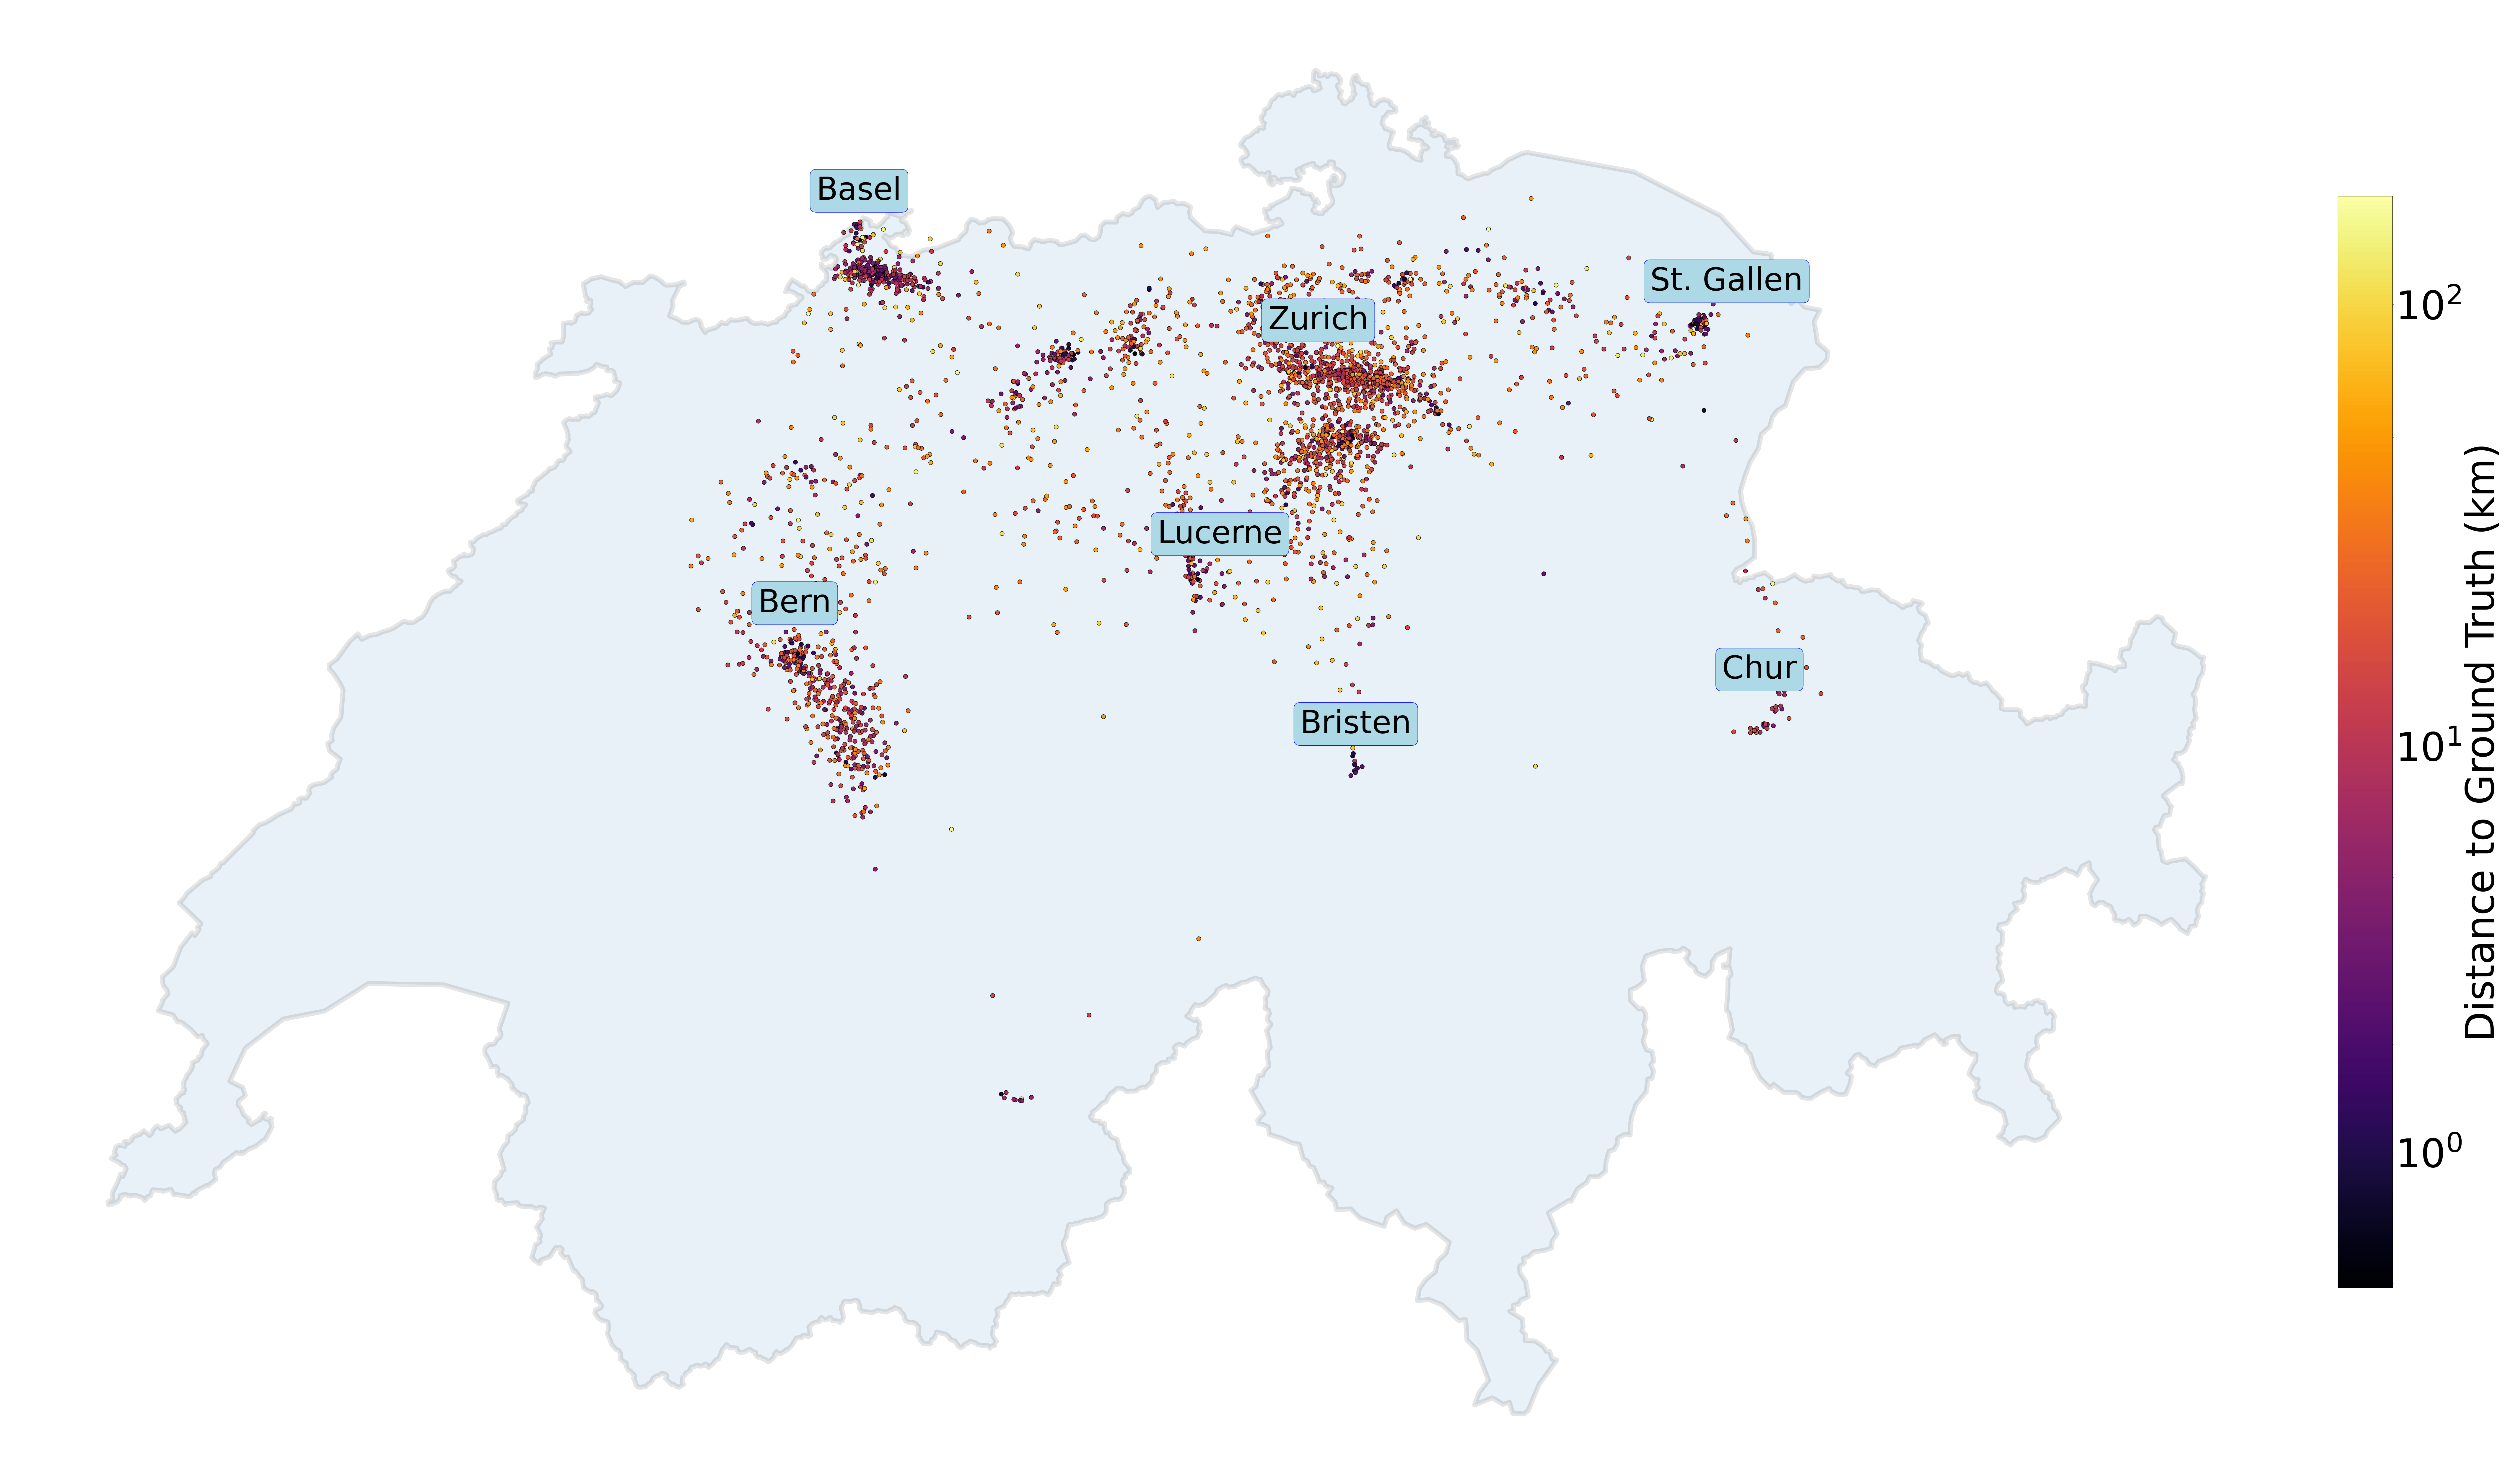
\includegraphics[width=\textwidth]{./figs/dotmap.png}
    \caption{Pointwise distance from the ground truth}
    \label{fig:pointwise-distance}
\end{figure}

\begin{figure}
    \centering
    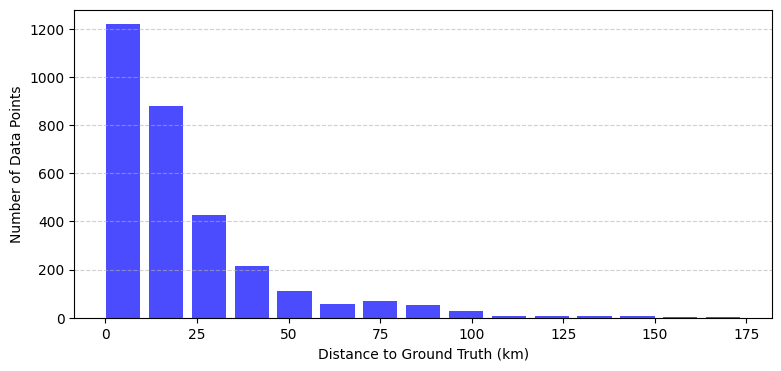
\includegraphics[width=\textwidth]{./figs/barchart.png}
    \caption{Error distribution: distances from predicted locations to ground truth}
    \label{fig:error-distribution}
\end{figure}

